\documentclass[border=12pt]{standalone}
\def\pgfsysdriver{pgfsys-dvisvgm.def}
\usepackage[dvisvgm]{xcolor}
\usepackage{xeCJK}
\setCJKmainfont{HaranoAjiGothic-Regular.otf}[BoldFont=HaranoAjiGothic-Bold.otf]
\setCJKsansfont{HaranoAjiGothic-Regular.otf}[BoldFont=HaranoAjiGothic-Bold.otf]
\usepackage{amsmath,amssymb,tikz,lmodern}
\usetikzlibrary{arrows.meta,positioning,calc,fit,backgrounds}
\renewcommand{\familydefault}{\sfdefault}
\definecolor{ink}{HTML}{25322F}
\definecolor{green}{HTML}{246657}
\definecolor{tint}{HTML}{EEF4F0}
\definecolor{soft}{HTML}{C6D2CC}
\definecolor{muted}{HTML}{52615B}
\newif\ifJapanese
\newcommand{\Tx}[2]{\ifJapanese #1\else #2\fi}
\newcommand{\Eff}{\overline{\operatorname{Eff}}}
\newcommand{\heading}[3]{{\color{green}\bfseries #1\quad\Tx{#2}{#3}}\\[5pt]}
% A white rectangle makes the complete citation label clickable, including spaces.
\newcommand{\refurl}[2]{\special{dvisvgm:raw <a xlink:href="#1" target="_blank" rel="noopener noreferrer">}{\setlength{\fboxsep}{0pt}\colorbox{white}{\color{green}\underline{\strut #2}}}\special{dvisvgm:raw </a>}}
\newcommand{\refedge}[3]{\refurl{\csname source#1\endcsname\string##page=#2}{#3}}
\newcommand{\SF}[2]{\refedge{sf}{#1}{#2}}
% GitHub's file preview does not support PDF page fragments.
\newcommand{\LA}[2]{\refurl{\sourcela}{#2}}
\newcommand{\Sch}[2]{\refedge{sch}{#1}{#2}}
\newcommand{\PS}[2]{\refedge{ps}{#1}{#2}}
\tikzset{
 card/.style={draw=soft,fill=white,rounded corners=2pt,align=left,text=ink,font=\fontsize{10.5}{14}\selectfont,inner xsep=12pt,inner ysep=10pt,text width=14.4cm},
 half/.style={card,text width=6.45cm,minimum height=2.05cm},
 result/.style={card,draw=green,fill=tint,line width=.9pt},
 reason/.style={align=left,text=muted,font=\fontsize{9}{12}\selectfont,inner sep=0pt,text width=12.7cm},
 branchreason/.style={reason,text width=5.95cm},
 edge/.style={-{Stealth[length=2.4mm]},draw=green,line width=1pt},
 wire/.style={draw=green,line width=1pt},
}
% Keep the arrow in a dedicated left gutter; explanations never cover it.
\newcommand{\flow}[3]{
 \coordinate (#2-from) at ($(#1.south)+(-6.9,0)$);
 \coordinate (#2-to) at ($(#2.north)+(-6.9,0)$);
 \draw[edge] (#2-from)--(#2-to);
 \node[reason,anchor=west] (#2-reason) at ($(#2-from)!.5!(#2-to)+(.55,0)$) {#3};
}

\Japanesetrue
\newcommand{\sourcesf}{https://raw.githubusercontent.com/openai/math/adc7f1241b42e322a6451854ab7e4b4c146bf78a/preprints/Schnell-fiber-spaces-and-good-canonical-models-September-24-2026/paper.pdf}
\newcommand{\sourcela}{https://github.com/openai/math/blob/adc7f1241b42e322a6451854ab7e4b4c146bf78a/preprints/Log-abundance-in-characteristic-zero-September-24-2026/paper.pdf}
\newcommand{\sourcesch}{https://arxiv.org/pdf/2202.01295v1}
\newcommand{\sourceps}{https://arxiv.org/pdf/1405.6125v2}
\begin{document}
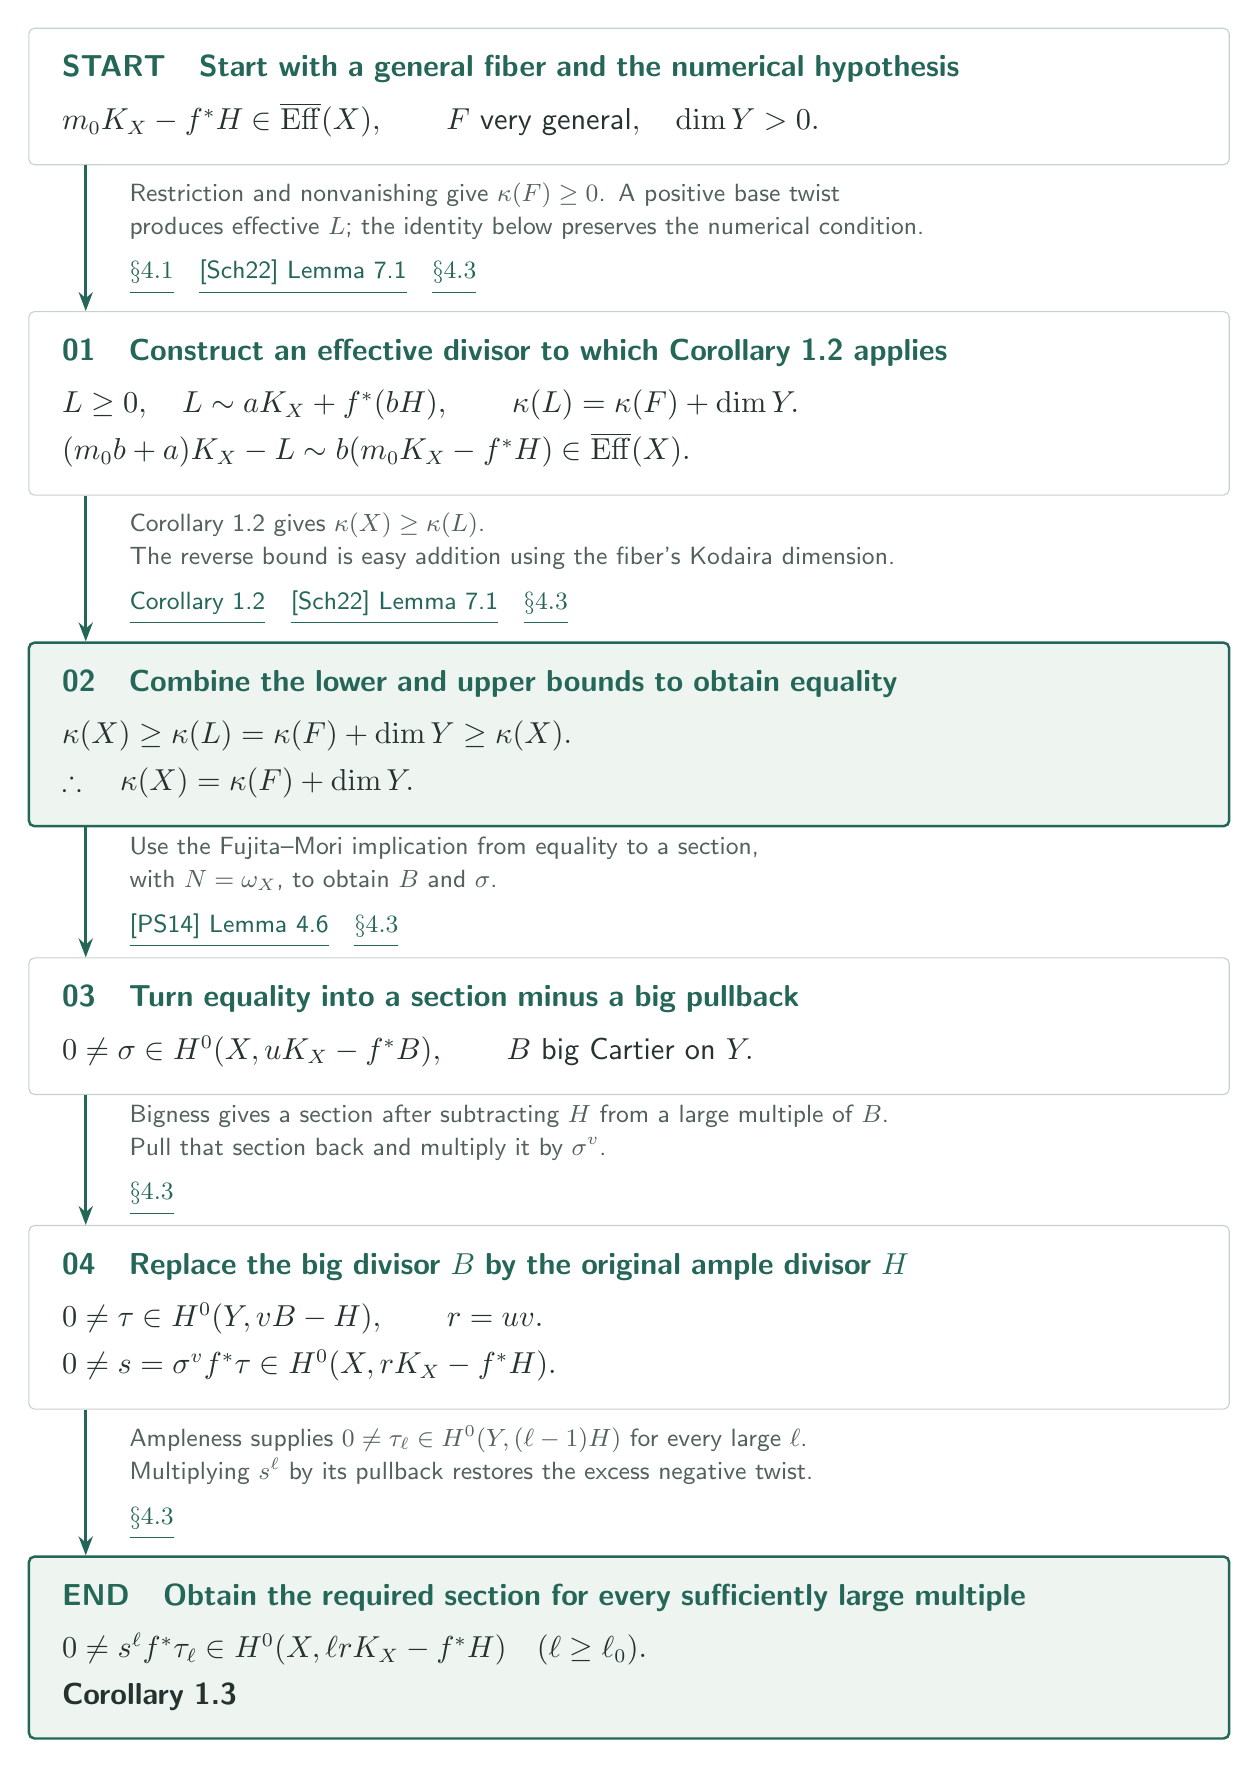
\begin{tikzpicture}
\node[card] (input) {\heading{START}{一般のファイバーで、数値的仮定から出発する}{Start with a general fiber and the numerical hypothesis}
$m_0K_X-f^*H\in\Eff(X),\qquad F\text{ very general},\quad\dim Y>0.$};
\node[card,below=1.85cm of input] (effective) {\heading{01}{Corollary 1.2を適用できる有効因子を作る}{Construct an effective divisor to which Corollary 1.2 applies}
$L\ge0,\quad L\sim aK_X+f^*(bH),\qquad\kappa(L)=\kappa(F)+\dim Y.$\\[3pt]
$(m_0b+a)K_X-L\sim b(m_0K_X-f^*H)\in\Eff(X).$};
\flow{input}{effective}{\Tx{ファイバーへの制限と非消滅から $\kappa(F)\ge0$。\\正の底の捻りで有効な $L$ を作り、数値的仮定を恒等式で引き継ぐ。}{Restriction and nonvanishing give $\kappa(F)\ge0$. A positive base twist\\produces effective $L$; the identity below preserves the numerical condition.}\\[4pt]\SF{8}{$\S4.1$}\quad\Sch{3}{[Sch22] Lemma 7.1}\quad\SF{10}{$\S4.3$}}
\node[result,below=1.85cm of effective] (equality) {\heading{02}{下界と上界を合わせ、小平次元の等式を得る}{Combine the lower and upper bounds to obtain equality}
$\kappa(X)\ge\kappa(L)=\kappa(F)+\dim Y\ge\kappa(X).$\\[3pt]
$\therefore\quad\kappa(X)=\kappa(F)+\dim Y.$};
\flow{effective}{equality}{\Tx{Corollary 1.2 は $\kappa(X)\ge\kappa(L)$ を与える。\\逆向きは、ファイバーの小平次元による easy addition の上界。}{Corollary 1.2 gives $\kappa(X)\ge\kappa(L)$.\\The reverse bound is easy addition using the fiber's Kodaira dimension.}\\[4pt]\SF{2}{Corollary 1.2}\quad\Sch{3}{[Sch22] Lemma 7.1}\quad\SF{10}{$\S4.3$}}
\node[card,below=1.65cm of equality] (big) {\heading{03}{等式を、底のbig因子を引いた切断の存在へ変える}{Turn equality into a section minus a big pullback}
$0\ne\sigma\in H^0(X,uK_X-f^*B),\qquad B\text{ big Cartier on }Y.$};
\flow{equality}{big}{\Tx{Fujita--Mori判定の「小平次元の等式 $\Rightarrow$ 切断の存在」を\\$N=\omega_X$ に適用し、$B$ と $\sigma$ を得る。}{Use the Fujita--Mori implication from equality to a section,\\with $N=\omega_X$, to obtain $B$ and $\sigma$.}\\[4pt]\PS{14}{[PS14] Lemma 4.6}\quad\SF{10}{$\S4.3$}}
\node[card,below=1.65cm of big] (original) {\heading{04}{big因子 $B$ を、元の豊富因子 $H$ に置き換える}{Replace the big divisor $B$ by the original ample divisor $H$}
$0\ne\tau\in H^0(Y,vB-H),\qquad r=uv.$\\[3pt]
$0\ne s=\sigma^v f^*\tau\in H^0(X,rK_X-f^*H).$};
\flow{big}{original}{\Tx{$B$ のbig性より、十分な倍数から $H$ を引いても切断がある。\\その切断を引き戻し、$\sigma^v$ に掛ける。}{Bigness gives a section after subtracting $H$ from a large multiple of $B$.\\Pull that section back and multiply it by $\sigma^v$.}\\[4pt]\SF{10}{$\S4.3$}}
\node[result,below=1.85cm of original] (goal) {\heading{END}{十分大きいすべての倍数で、所要の切断を得る}{Obtain the required section for every sufficiently large multiple}
$0\ne s^\ell f^*\tau_\ell\in H^0(X,\ell rK_X-f^*H)\quad(\ell\ge\ell_0).$\\[3pt]\textbf{Corollary 1.3}};
\flow{original}{goal}{\Tx{$H$ の豊富性より、すべての十分大きな $\ell$ に対して\\$0\ne\tau_\ell\in H^0(Y,(\ell-1)H)$。$s^\ell$ に掛け、余分な捻りを戻す。}{Ampleness supplies $0\ne\tau_\ell\in H^0(Y,(\ell-1)H)$ for every large $\ell$.\\Multiplying $s^\ell$ by its pullback restores the excess negative twist.}\\[4pt]\SF{10}{$\S4.3$}}
\end{tikzpicture}

\end{document}
